\section{Anhang}


\vspace{1em}
\begin{table}[H]
\centering
\begin{tabular}{|p{4.5cm}|p{9.5cm}|}
\hline
\textbf{Komponente} & \textbf{Spezifikation} \\
\hline
Gerätetyp & Laptop \\
\hline
Hersteller & HP \\
\hline
Modell & Pavilion Laptop 14-bf0xx \\
\hline
Prozessor (CPU) & Intel\textsuperscript{\textregistered} Core\texttrademark\ i5-7200U CPU mit 2,50\,GHz, 2 Kerne, 4 Threads \\
\hline
Arbeitsspeicher (RAM) & 8\,GB (1x 8\,GB, DDR4, 2133\,MHz, SODIMM, SK Hynix) \\
\hline
Grafikeinheit (GPU) & Intel HD Graphics 620 (integriert) \newline NVIDIA GeForce 940MX (dediziert) \\
\hline
Massenspeicher & Samsung SSD 256\,GB \\
\hline
Betriebssystem & Linux Mint 21.3 „Virginia“ (64-bit) \\
\hline
\end{tabular}
\caption{Technische Spezifikationen des Testsystems „System B LT“}
\label{tab:system_b_lt}
\end{table}
\vspace{1em}








\vspace{1em}
\begin{table}[H]
\centering
\begin{tabular}{|p{4.5cm}|p{9.5cm}|}
\hline
\textbf{Komponente} & \textbf{Spezifikation} \\
\hline
Gerätetyp & Workstation (Micro Form Factor) \\
\hline
Hersteller & Dell \\
\hline
Modell & OptiPlex 7000 Micro \\
\hline
Prozessor (CPU) & Intel\textsuperscript{\textregistered} Core\texttrademark\ i5-12500T CPU mit 2,00–4,60\,GHz, 6 Kerne, 12 logische Prozessoren \\
\hline
Arbeitsspeicher (RAM) & 16\,GB DDR4 (1× 16\,GB, 3200\,MHz, SODIMM) \\
\hline
Grafikeinheit (GPU) & Integrierte Intel UHD Graphics 770 \\
\hline
Massenspeicher & 256\,GB NVMe SSD (PCIe 3.0 x4, M.2) \\
\hline
Betriebssystem & Windows 11 Pro (64-bit), Version 22H2 (Build 22621) \\
\hline
\end{tabular}
\caption{Technische Spezifikationen des Testsystems „System C WS“}
\label{tab:system_c_ws}
\end{table}
\vspace{1em}







\vspace{1em}
\begin{table}[H]
\centering
\begin{tabular}{|p{4.5cm}|p{9.5cm}|}
\hline
\textbf{Komponente} & \textbf{Spezifikation} \\
\hline
Gerätetyp & Access Point (Indoor) \\
\hline
Hersteller & TP-Link \\
\hline
Modell & TL-WA801N \\
\hline
WLAN-Standard & IEEE 802.11n (2.4\,GHz) \\
\hline
Maximale Übertragungsrate & 300\,Mbit/s \\
\hline
Ethernet-Anschluss & 1× Fast Ethernet (10/100\,Mbit/s) \\
\hline
Antennen & 2× externe, abnehmbare Antennen \\
\hline
Betriebssystem & Eigenständige Firmware (Webinterface konfigurierbar) \\
\hline
\end{tabular}
\caption{Technische Spezifikationen des Testsystems „System D AP“}
\label{tab:system_d_ap}
\end{table}
\vspace{1em}






\vspace{1em}
\begin{table}[H]
\centering
\begin{tabular}{|p{4.5cm}|p{9.5cm}|}
\hline
\textbf{Komponente} & \textbf{Spezifikation} \\
\hline
Gerätetyp & Desktop \\
\hline
Hersteller & Eigenbau (ASUS-Mainboard, OEM-Konfiguration) \\
\hline
Prozessor (CPU) & Intel\textsuperscript{\textregistered} Core\texttrademark\ i7-9700K CPU mit 3,60\,GHz, 8 Kerne, 8 logische Prozessoren \\
\hline
Arbeitsspeicher (RAM) & 16\,GB (2x 8\,GB, 3000\,MHz, DIMM) \\
\hline
Grafikeinheit (GPU) & NVIDIA GeForce RTX 2070 \\
\hline
Massenspeicher & Samsung SSD 970 EVO Plus 500\,GB \\
\hline
Betriebssystem & Windows 10 Home (64-bit), Version 10.0.19045 Build 19045 \\
\hline
\end{tabular}
\caption{Technische Spezifikationen des Testsystems „System A DT“}
\label{tab:system_a_dt}
\end{table}
\vspace{1em}




\vspace{1em}
\begin{table}[H]
\centering
\begin{tabular}{|p{4.5cm}|p{9.5cm}|}
\hline
\textbf{Komponente} & \textbf{Spezifikation} \\
\hline
Gerätetyp & Virtuelle Maschine (KVM) \\
\hline
Prozessor (CPU) & AMD EPYC Processor, 3{,}0\,GHz, 8 Kerne, 8 Threads \\
\hline
Arbeitsspeicher (RAM) & 16\,GB \\
\hline
Cache & L1: 256\,KiB, L2: 4\,MiB, L3: 64\,MiB \\
\hline
Betriebssystem & Ubuntu 20.04.6 LTS (64-bit) \\
\hline
Kernel-Version & Linux 5.4.0-216-generic \\
\hline
Architektur & x86\_64 (64-bit) \\
\hline
Hypervisor & KVM \\
\hline
Virtualisierungstyp & Vollvirtualisierung \\
\hline
\end{tabular}
\caption{Technische Spezifikationen des Zielservers (JupyterHub-VM)}
\label{tab:jupyterhub_vm}
\end{table}
\vspace{1em}








\begin{figure}[H]
    \centering
    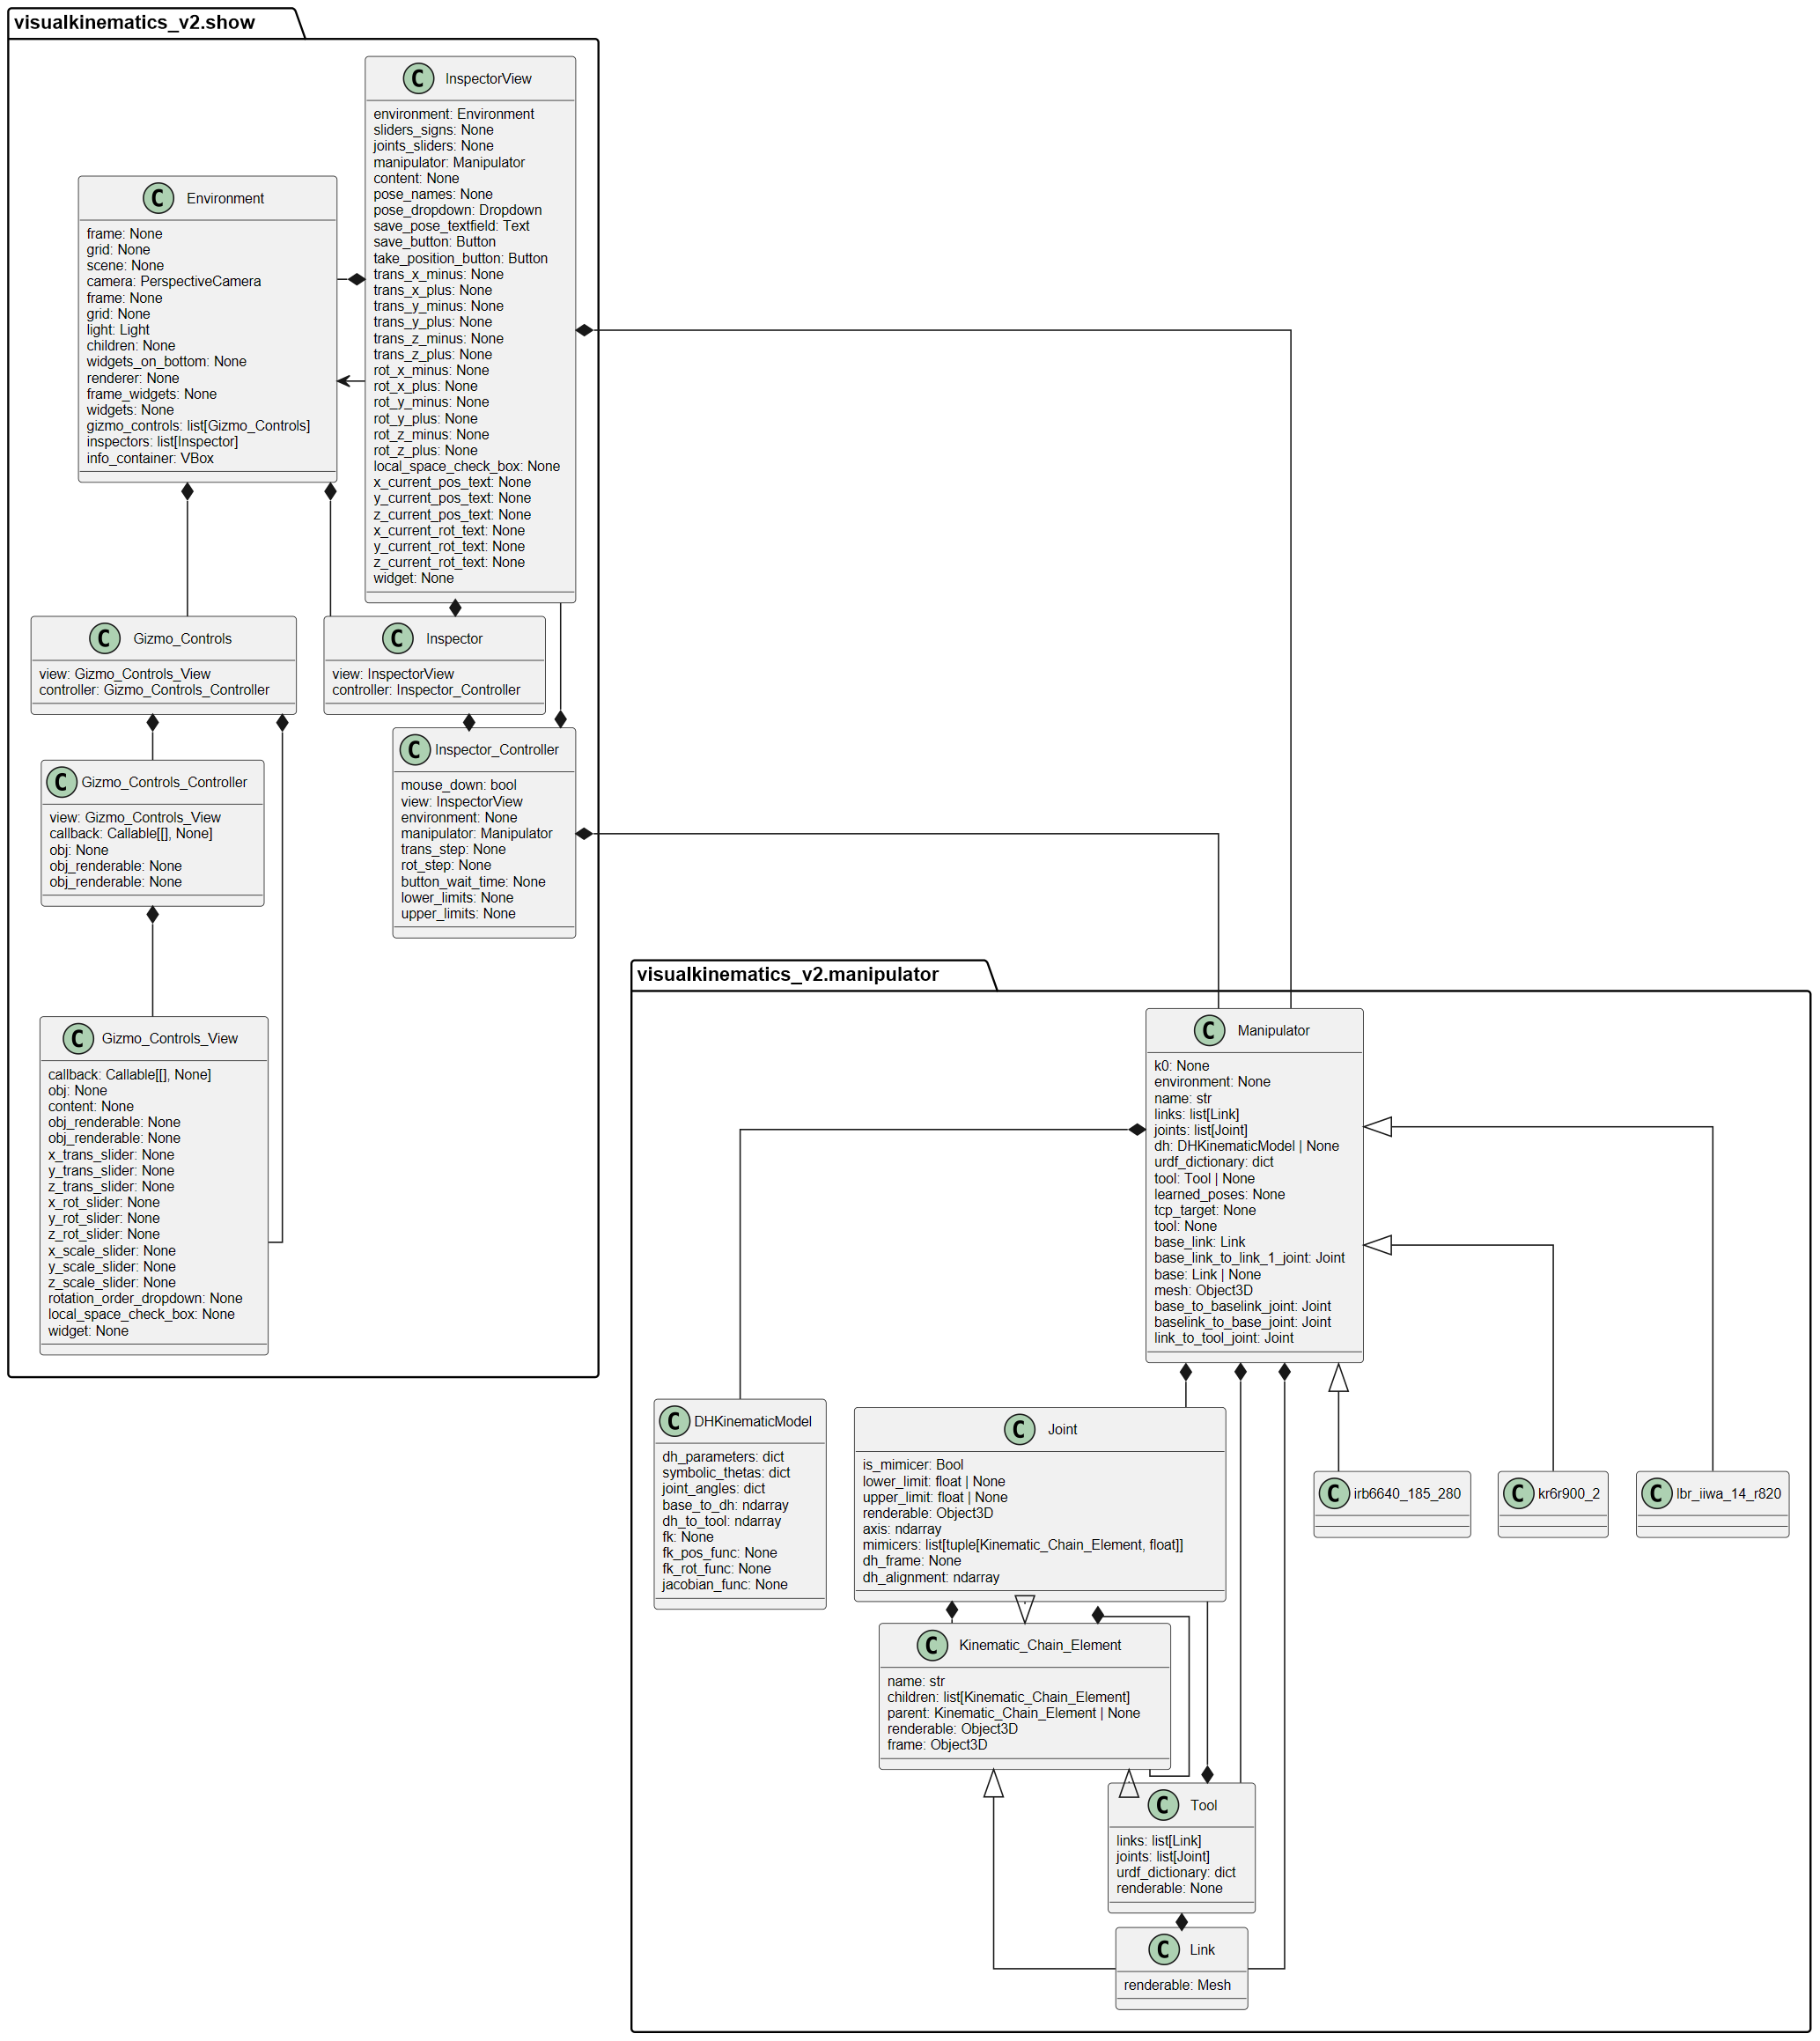
\includegraphics[width=1.0\textwidth]{images/class_diagramm.png}
    \caption{UML-Klassendiagramm des Frameworks generiert mit dem Tool py2puml}
    \label{fig:class_diagramm}
\end{figure}


\begin{figure}[H]
    \centering
    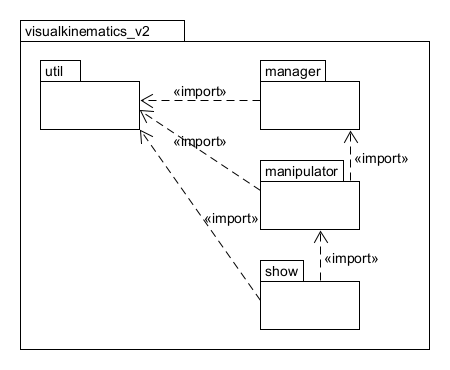
\includegraphics[width=0.75\textwidth]{images/package_diagramm.png}
    \caption{UML-Packagediagramm der Module}
    \label{fig:package_diagramm}
\end{figure}





